\section{Lernfeld 2 - Geschäftsprozesse und betriebliche Organisation}

\subsection{Projektmanagment}

Kriterien eines Projektes:
\begin{itemize}
	\item Einmaligkeit
	\item Zeitbegrenzung
	\item Bedeutsamkeit
	\item Komplexität
	\item Fachübergreifend
	\item Risiko
\end{itemize}

Anlässe für Projekte: Bsp.
\begin{itemize}
	\item Organisatorische Probleme: schlechter Informationsfluss
	\item Technische Probleme: hoher Wartungsaufwand
	\item Wirtschaftliche Probleme: sinkende Umsätze
	\item Marktbezogene Entwicklungen: Wettbewerbsdruck
	\item Innovation: neue Produktideen
	\item Controlling-Ergebnisse: ineffiziente Systeme
\end{itemize}

Magisches Dreieck des Projektmanagments:\\
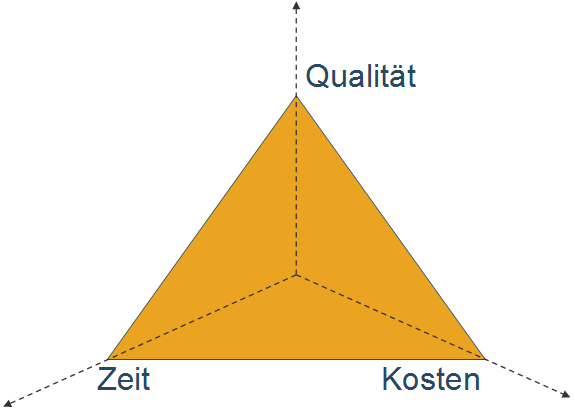
\includegraphics[scale=0.5]{pictures/lf02-pic/lf02-projekt-dreieck.png}

Wenn ein \textbf{Projektantrag} genehmigt wird, wird daraus ein \textbf{Projektauftrag}. Der Projektantrag enthält folgende Informationen:
\begin{itemize}
	 \item Aufgabenbeschreibung
	 \item Erwarteter Nutzen
	 \item Konsequenzen bei Nicht-Beachtung
	 \item Rahmenbedingungen
\end{itemize}
Projektauftrag:
\begin{itemize}
	\item Was soll realisiert werden?
	\item Welche Qualität wird angestrebt?
	\item Wie viel soll realisiert werden?
	\item Personal: wer wird eingesetzt?
	\item Material: womit wird die Realisierung erfolgen?
	\item Zeitrahmen: wie lange soll das Projekt dauern?
	\item Wo soll das Projekt umgesetzt werden?
	\item Welche Risiken bestehen?
\end{itemize}

\begin{itemize}
	\item Minimalprinzip
	\item Maximalprinzip
\end{itemize}


\subsection{Motivation}
- Herzberg
- Maslow

\subsection{Projektcontrolling}
\subsubsection{Balanced Scorecard}